\documentclass[Report.tex]{subfiles}
\begin{document}
This section describes the typical workflow of a data scientist. We will focus on the following four phases: Preparation, Analysis, Reflection and Dissemination.

The process of getting the data, understanding the data and producing results is an iterative process. The process can be seen on Figure \ref{Fig:Iterative}.

\begin{figure}
\center
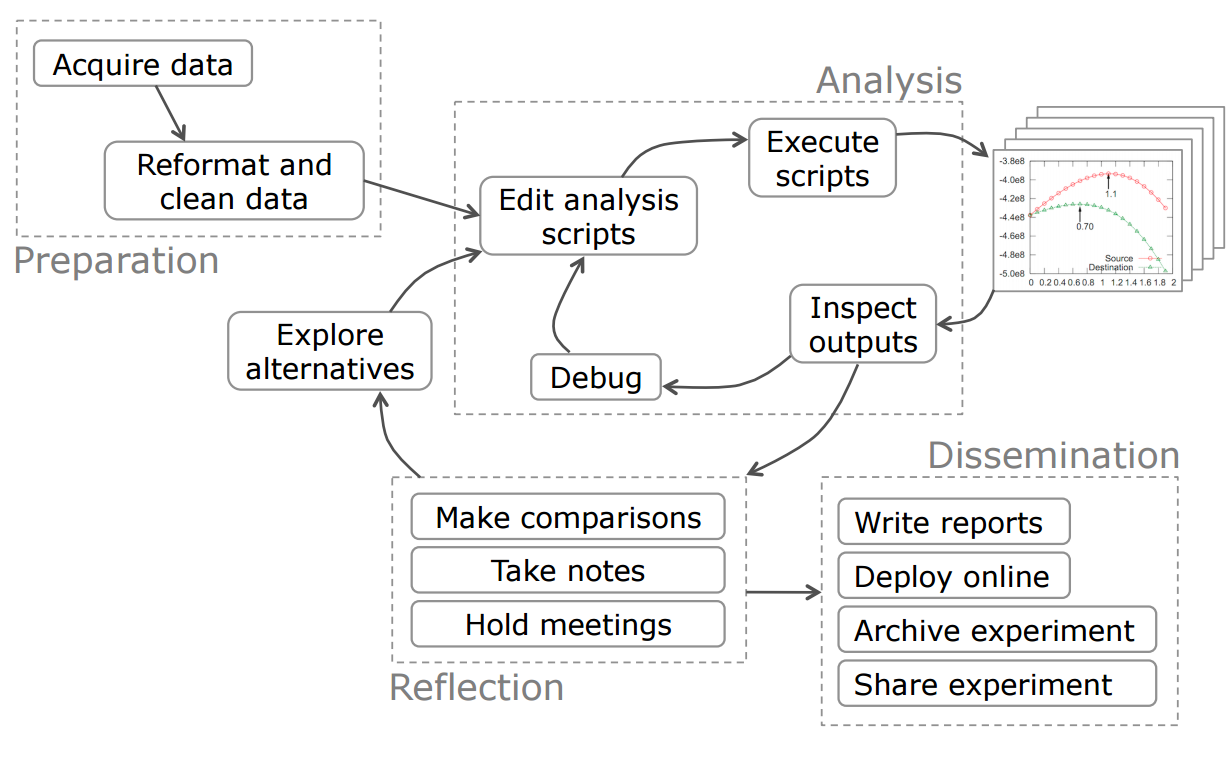
\includegraphics[scale=0.4]{Iterative.png}
\caption{The model showing the iterative process\cite[Chapter 2]{Guo}}
\label{Fig:Iterative}
\end{figure}
\begin{itemize}


\item The first phase is the preparation phase. Here the data is acquired, which could be from hard disk, server, through an API etc. Where to store and how to organize the data files should also be considered, to allow easy replacement of the right files should the data be updated. Hereafter the data should be cleaned, which includes removing tuples with missing values, changing the formatting, sorting the data etc.


\item The second phase is the analysis phase. Here the data is analysed to get more information. This is an iterative process, where you create and run scripts,  look at the output, correct eventual errors, debug these and run it again. 

\item The third phase is the reflection phase. Here the output results are discussed, for example by making comparisons between outputs, and exploring alternatives.

\item The fourth and last phase is the dissemination phase. Here the results are reported and possibly published in a report.
\cite[Chapter 2]{Guo}


\end{itemize}

\end{document}